\documentclass[conference]{IEEEtran}
\IEEEoverridecommandlockouts
\usepackage{float}
\usepackage{cite}
\usepackage{amsmath,amssymb,amsfonts}
\usepackage{algorithmic}
\usepackage{graphicx}
\usepackage{textcomp}
\usepackage{xcolor}
\usepackage{subcaption}
\usepackage{url}

\def\BibTeX{{\rm B\kern-.05em{\sc i\kern-.025em b}\kern-.08em
    T\kern-.1667em\lower.7ex\hbox{E}\kern-.125emX}}

\begin{document}

\title{AI-Assisted Colorimetric Analysis for Antibiotic Susceptibility Testing: Final Project Report and Inferences}

\author{
  \IEEEauthorblockN{Ashwath}
  \IEEEauthorblockA{\textit{Dept. of Artificial Intelligence} \\
  \textit{IIT Hyderabad}\\
  Hyderabad, India}
  \and
  \IEEEauthorblockN{Vardhan}
  \IEEEauthorblockA{\textit{Dept. of Engineering Science} \\
  \textit{IIT Hyderabad}\\
  Hyderabad, India}
}

\maketitle

\begin{abstract}
Standard Antibiotic Susceptibility Testing (AST) is often hindered by the high cost of microplate readers, particularly in resource-limited settings. In this work, we propose a cost-effective alternative using computer vision and smartphone-based image acquisition. By utilizing the Resazurin colorimetric indicator, which shifts from blue/purple to pink (Resorufin) in the presence of bacterial metabolic activity, we develop a robust analytical pipeline. Our approach combines Signal-Guided Machine Learning (ML) for fluid segmentation using the Segment Anything Model (SAM) and CIELAB color space quantification for precise tracking of "Pinkness". Statistical distribution analysis via Jensen-Shannon Distance (JSD) and Kolmogorov-Smirnov (KS) tests provides a probabilistic framework for Minimum Inhibitory Concentration (MIC) determination. The results demonstrate that our computer vision-based method effectively tracks bacterial growth inhibition across dilution series, offering a promising path toward decentralized point-of-care diagnostics.
\end{abstract}

\begin{IEEEkeywords}
Antibiotic Susceptibility Testing (AST), Resazurin, Computer Vision, SAM, CIELAB, Statistical Analysis, Point-of-Care.
\end{IEEEkeywords}

\section{Introduction}
Antibiotic Susceptibility Testing (AST) is critical for determining the Minimum Inhibitory Concentration (MIC) of antibiotics against specific bacterial strains. Traditional methods, while accurate, often rely on expensive equipment such as microplate readers, which can cost upwards of Rs. 10 Lakhs. This financial barrier limits the accessibility of AST in rural and resource-constrained environments.

To address this, colorimetric assays using Resazurin have been developed. Resazurin is a blue non-fluorescent dye that is reduced to pink and highly fluorescent Resorufin by the metabolic activity of living cells. While visual inspection can provide a qualitative assessment, it is subjective and prone to human error.

In this work, we present an automated computer vision pipeline designed to quantify the colorimetric shift in Resazurin-based assays. The goal is to standardize the analysis on vials and well-plates, providing a foundation for transitioning to Freeze-Dried Bacterial Cellulose (FDBC) substrates for rapid, point-of-care diagnostics.

\section{Methodology}

\subsection{Image Acquisition and Pre-processing}
Images of the experimental setup were captured using a smartphone camera. For the vials, the layout consisted of a 2x10 grid, where the first row (Row 1) served as a dye control (sterility check), while the second row (Row 2) contained bacteria with a decreasing concentration of antibiotics (128, 64, 32, 16, 8, 4, 2, 1, 0.5, 0.25 $\mu$g/mL). 

Additionally, experiments were conducted using well-plates. The well-plates utilized a specific layout configuration containing rows of 10, 10, 10, 6, and 6 wells respectively (10/10/10/6/6). In this plate layout, the lower-right 2x3 wells served as a media-only control, which was critical for global reference extraction and establishing baseline statistics. 

Pre-processing involved automated grid and circle detection. While Hough Transforms were initially explored (and specifically applied locally within Regions of Interest for well-plate circle detection), a more robust "Signal-Guided" approach was implemented to handle varying lighting and background conditions.

\subsection{Segmentation: Signal-Guided ML}
Isolating the fluid regions from the vials and wells is challenging due to reflections and the transparency of the containers. We utilized the \textbf{HSV Saturation channel} to generate high-confidence seeds for fluid locations, as the colored fluid typically exhibits higher saturation than the background. 

These seeds were used as prompts for the \textbf{Segment Anything Model (SAM)}. By providing SAM with localized point prompts and bounding boxes derived from the saturation peaks, we achieved precise masks for each fluid region, minimizing "leaking" into the container boundaries.

\subsection{Quantification: CIELAB a* Channel}
To quantify the transition from blue to pink, we transformed the RGB images into the \textbf{CIELAB color space}. The \textbf{$a^*$ channel}, which represents the green-to-red axis, provides a robust measure of "Pinkness". Unlike RGB or intensity-based measures, the $a^*$ value is relatively independent of brightness, making it ideal for varying lighting environments. The median $a^*$ value within each segmented mask was extracted as the primary analytical metric.

\subsection{Normalization Using Layout-Based $a^*$ Affine Normalization}
To further mitigate environmental lighting variance, we implemented \textbf{layout-based affine normalization}. For well-plates, the $a^*$ intensity was normalized at each timepoint using the fixed plate layout and the control wells (the lower-right 2x3 media-only wells) to account for lighting conditions from image to image. For the FDBC, the $a^*$ values of the bacteria row were normalized using the sterility control row (Row 1).

To account for varying lighting conditions from image to image, a well-wise $a^*$ intensity affine normalization is applied at each timepoint. The normalization utilizes a fixed plate layout and extracts references from the media-only control wells (specifically, the lower-right $2 \times 3$ wells).

\subsubsection{Global Reference Statistics Extraction}
Only fully complete layouts (e.g., 10/10/10/6/6) contribute to the global reference statistics. We compute the following parameters:
\begin{itemize}
    \item $\mu_{all}$: The global mean of the reference values.
    \item $\sigma_{all}$: The global target spread, defined as the mean of the per-timepoint reference standard deviations.
\end{itemize}

\subsubsection{Per-Timepoint Affine Normalization}
For each timepoint $t$, local reference statistics are extracted from the control samples at that specific timepoint:
\begin{itemize}
    \item $\mu_t$: The mean of the reference samples at timepoint $t$.
    \item $\sigma_t$: The standard deviation of the reference samples at timepoint $t$.
\end{itemize}

Using these values, a scaling factor ($s_t$) and an offset ($b_t$) are calculated for the timepoint $t$:

\begin{equation}
    s_t = 
    \begin{cases} 
        \frac{\sigma_{all}}{\sigma_t} & \text{if } \sigma_t \neq 0 \\ 
        1 & \text{if } \sigma_t = 0 
    \end{cases}
\end{equation}

\begin{equation}
    b_t = \mu_{all} - s_t \mu_t
\end{equation}

Finally, the normalized $a^*$ intensity value, denoted as $a^*_{norm}$, is computed for every sample at timepoint $t$ by applying the scale and offset to the original $a^*$ value:
\begin{equation}
    a^*_{norm} = s_t \cdot a^* + b_t
\end{equation}

\begin{figure}[H]
\centering
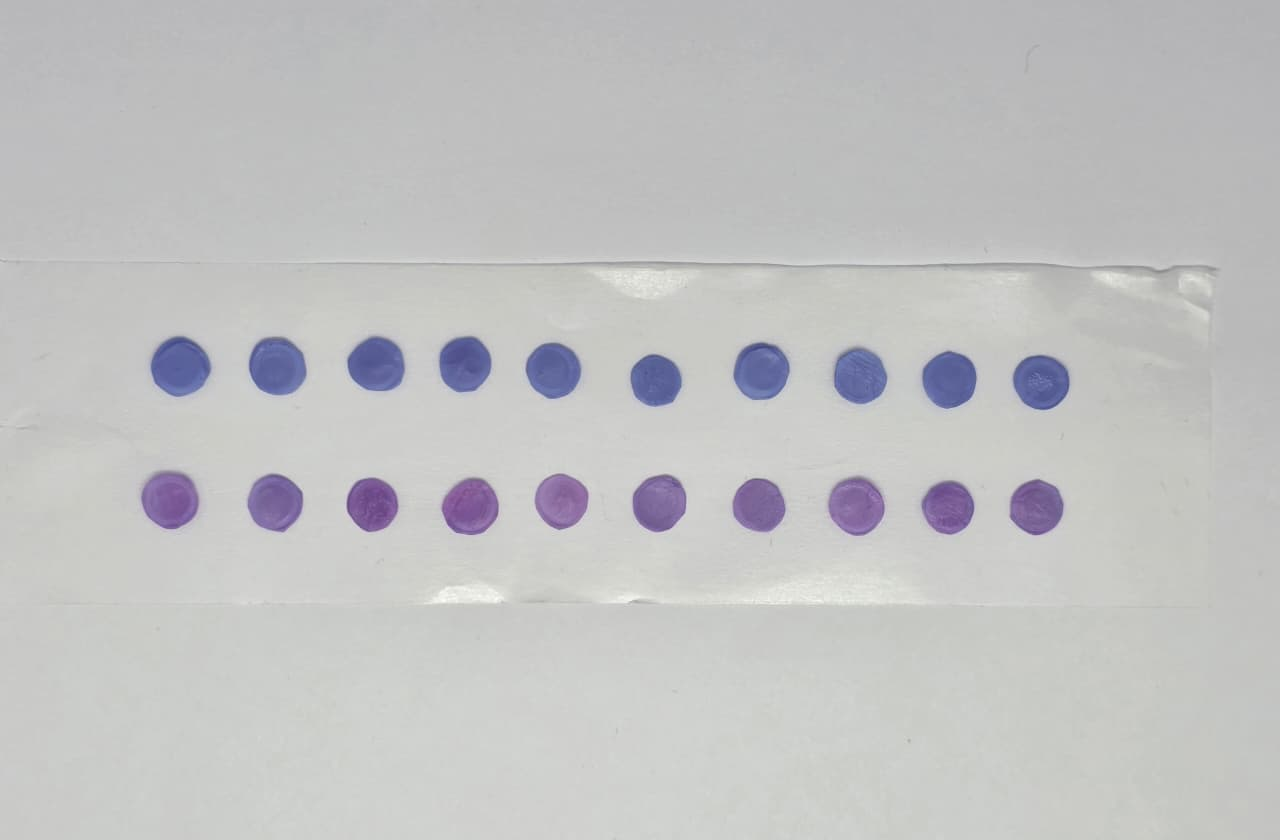
\includegraphics[width=0.48\textwidth]{samples/control/30th_min.png}
\caption{FDBC sample (30th minute) on which the normalization method was applied.}
\label{fig:fdbc_sample}
\end{figure}

\begin{figure}[H]
\centering
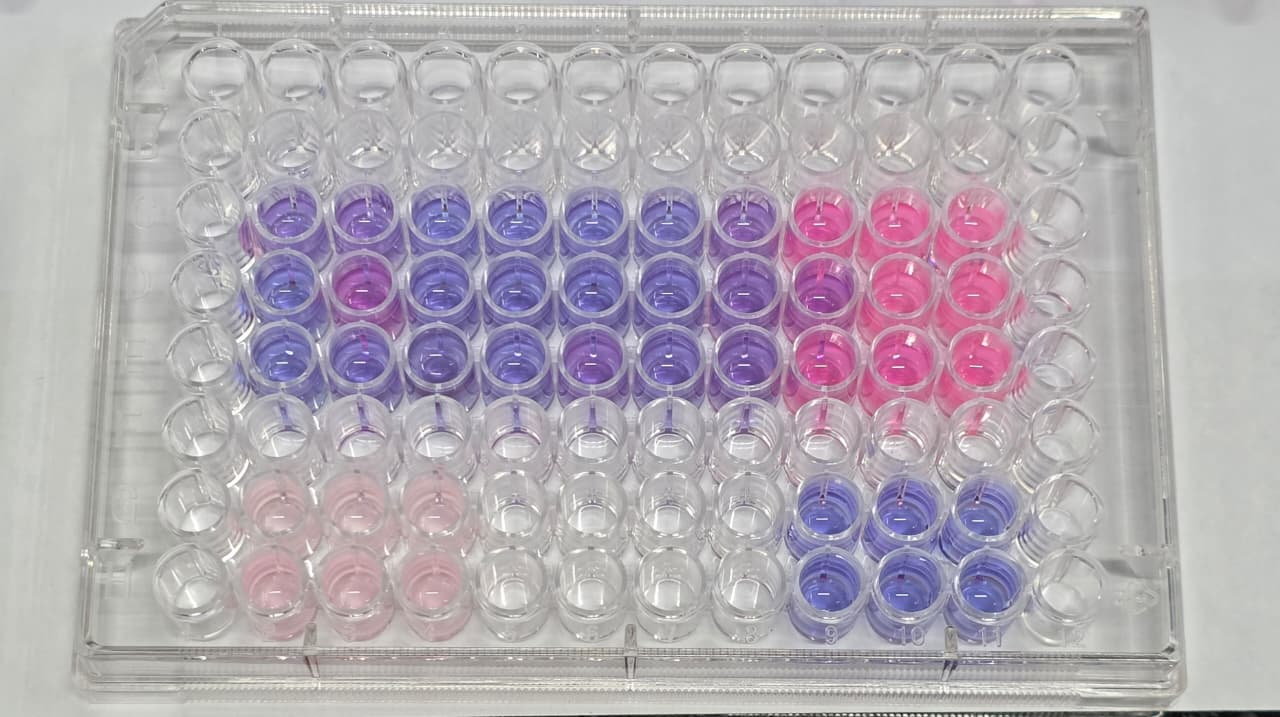
\includegraphics[width=0.48\textwidth]{samples/well_plate/70th_min.jpeg}
\caption{Well-plate sample (70th minute) on which the normalization method was applied.}
\label{fig:wp_sample}
\end{figure}

\subsection{Normalization and Statistical Tracking}
Statistical significance was assessed using:
\begin{itemize}
    \item \textbf{Jensen-Shannon Distance (JSD)}: To quantify the divergence between probability distributions of $a^*$ values across timepoints.
    \item \textbf{Kolmogorov-Smirnov (KS) Test}: To determine if the distribution of a sample at time $t$ is significantly different from time $t=0$, indicating growth.
\end{itemize}

\section{Results}

\subsection{Segmentation Accuracy}
The Signal-Guided ML approach successfully isolated the fluid regions across all timepoints. Fig. \ref{fig:segmentation} shows the segmentation overlay for the 60-minute mark, demonstrating the precision of the SAM-generated masks.

\begin{figure}[H]
\centering
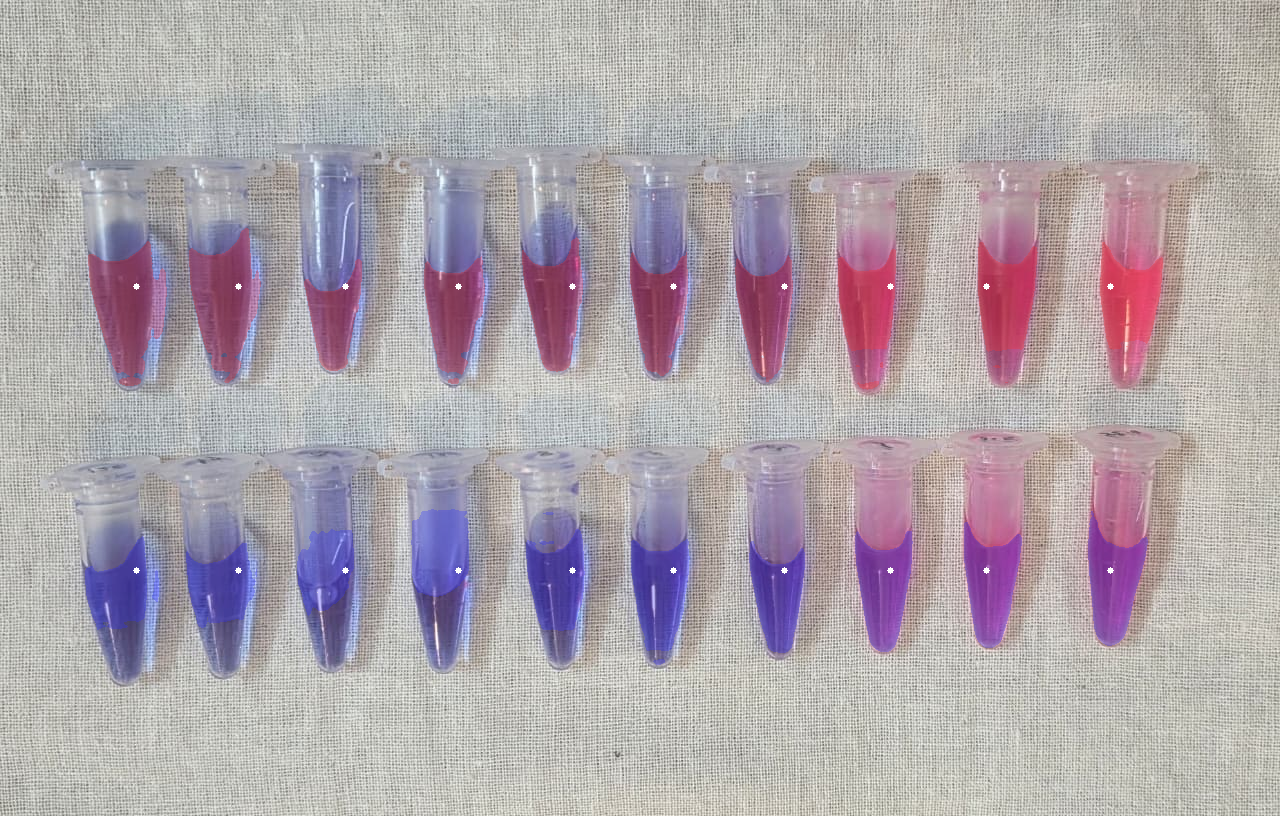
\includegraphics[width=0.48\textwidth]{results/broth/min60_overlay.png}
\caption{Segmentation overlay using SAM guided by HSV saturation prompts (60 min).}
\label{fig:segmentation}
\end{figure}

\subsection{Growth Kinetics and MIC Determination}
The "Pinkness" (median $a^*$) was tracked over time for each antibiotic concentration. As shown in Fig. \ref{fig:pinkness}, lower antibiotic concentrations exhibited a rapid increase in $a^*$, corresponding to bacterial growth and Resazurin reduction. Conversely, high concentrations remained relatively flat, indicating inhibition.

\begin{figure}[H]
\centering
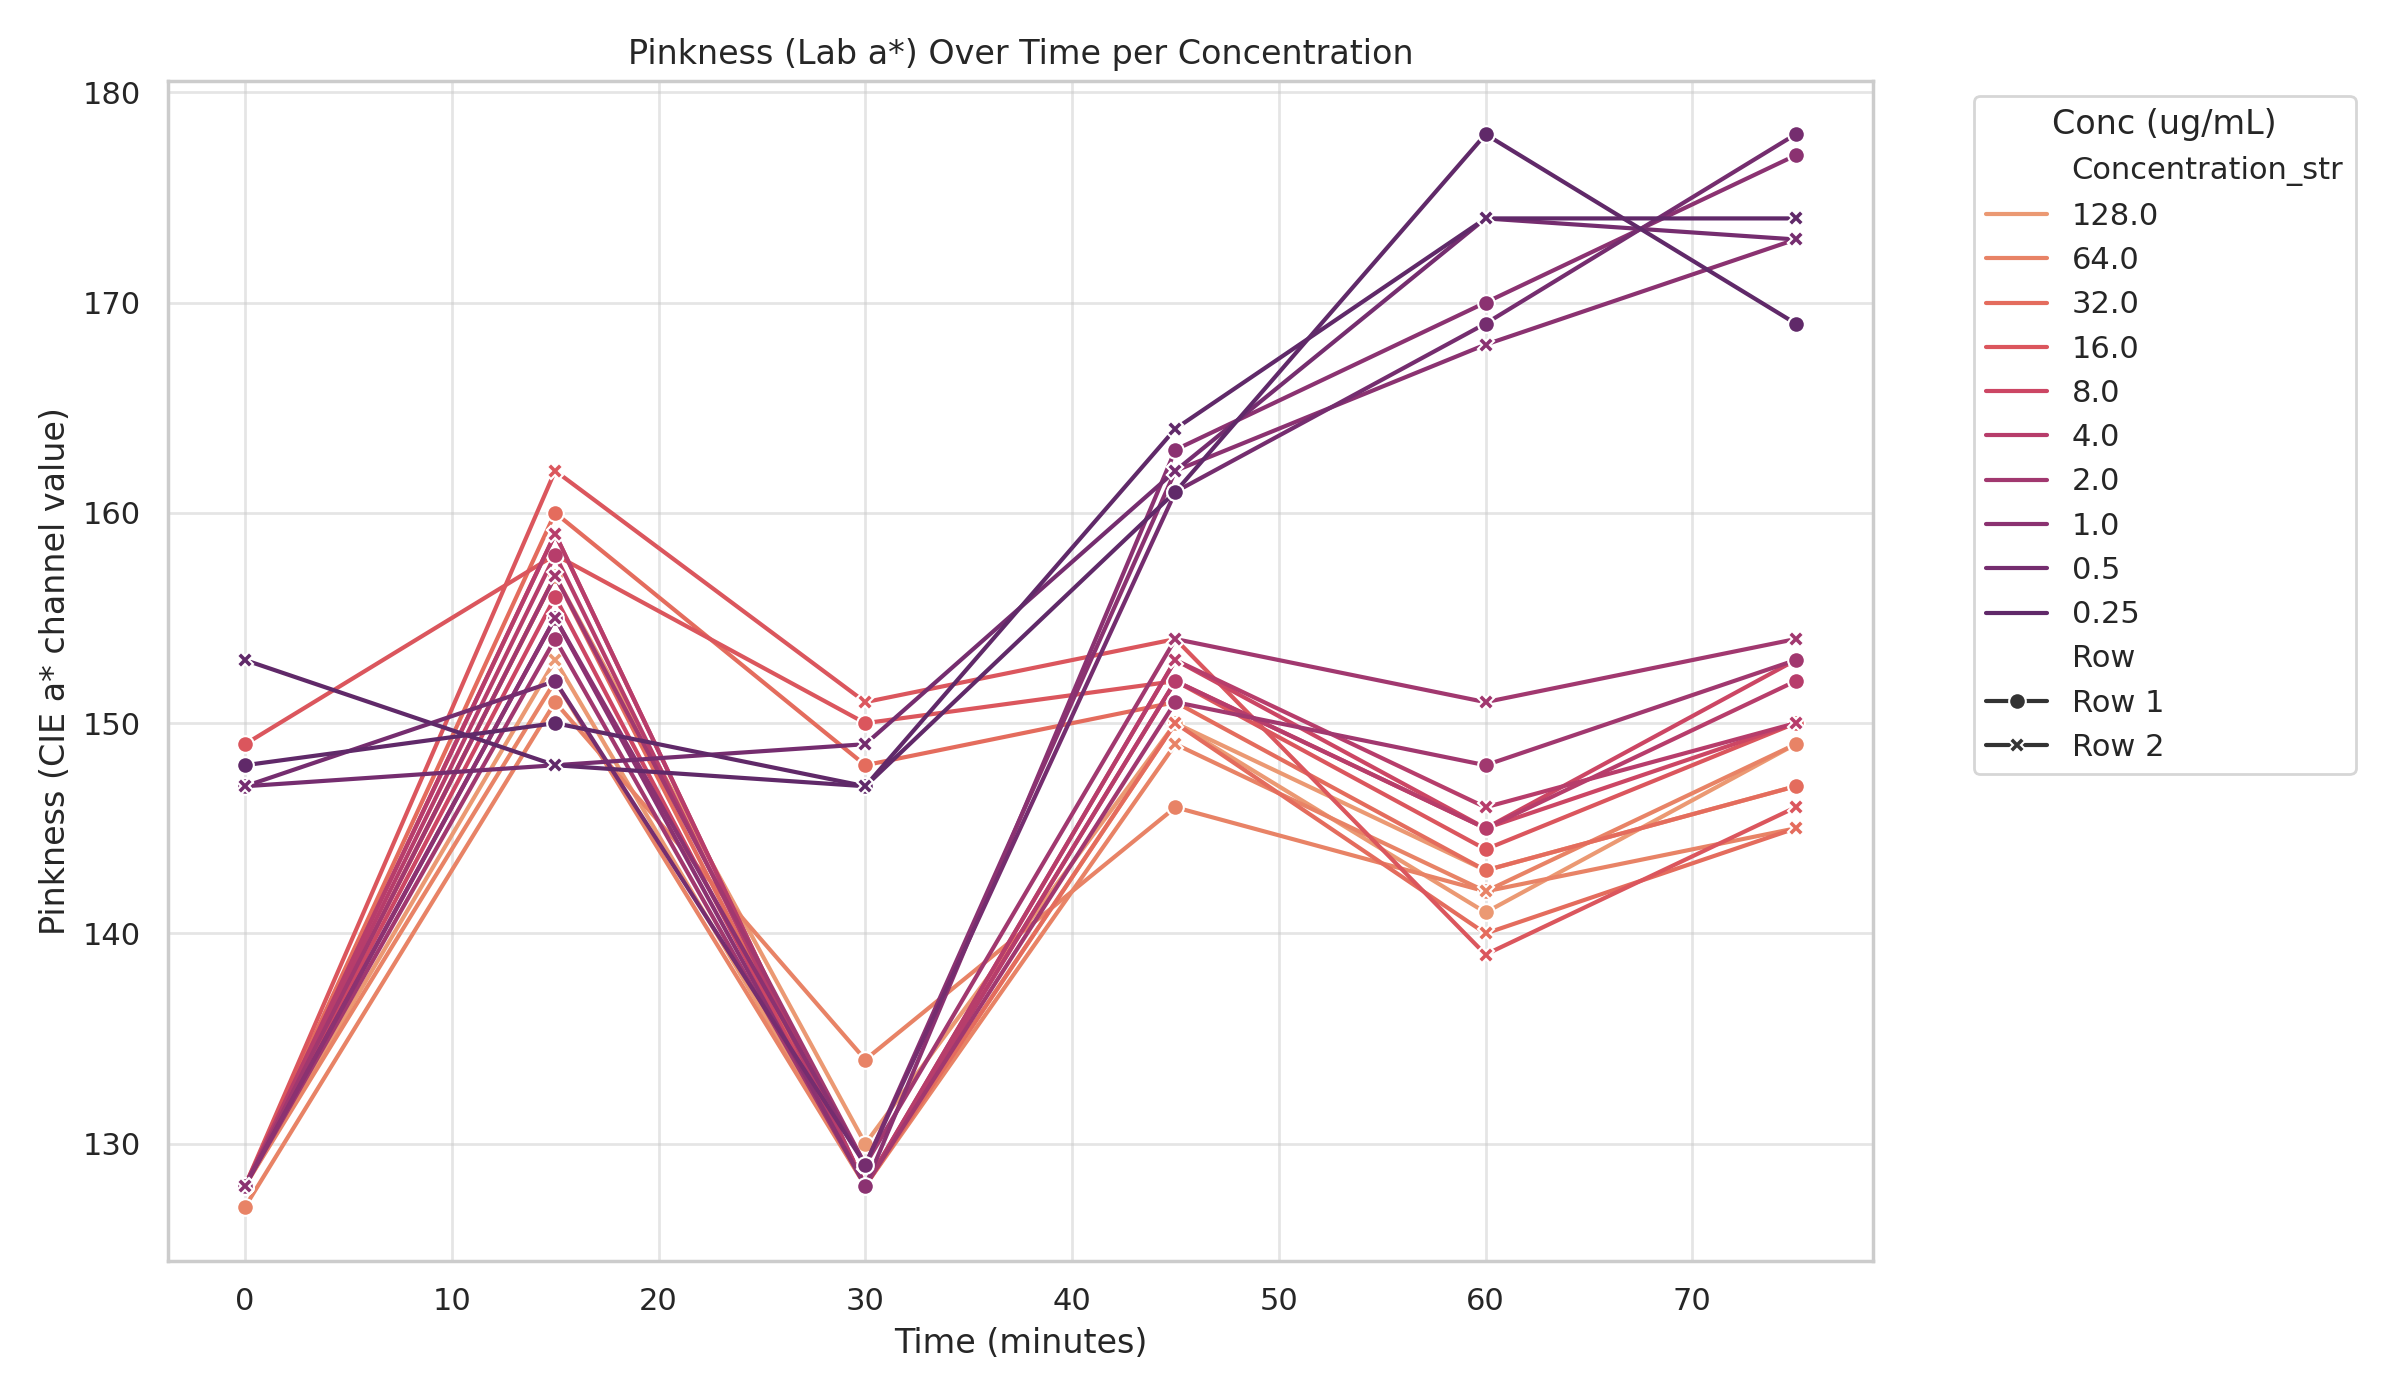
\includegraphics[width=0.48\textwidth]{results/analysis/pinkness_over_time.png}
\caption{Pinkness ($a^*$ channel) evolution over time for different antibiotic concentrations.}
\label{fig:pinkness}
\end{figure}

\subsection{Impact of Lighting Control and Normalization}

\subsubsection{Freeze-Dried Bacterial Cellulose (FDBC) Assays}
The necessity of the proposed affine normalization is clearly demonstrated in the FDBC experimental data. Without normalization, the sterility control row exhibits artificial fluctuations in color over time due to varying ambient lighting conditions (as shown in Fig. \ref{fig:fdbc_no_norm}). Since the control row should ideally maintain a constant colorimetric baseline, this variance highlights the susceptibility of raw image data to environmental noise.

Following the application of the normalization pipeline, these lighting-induced variances are successfully corrected. However, despite the normalization, the biological trends on FDBC discs remained inconsistent across trials. The normalized data for the bacteria-only row often failed to show a reliable dose-response curve compared to the well-plate experiments.

\begin{figure}[H]
\centering
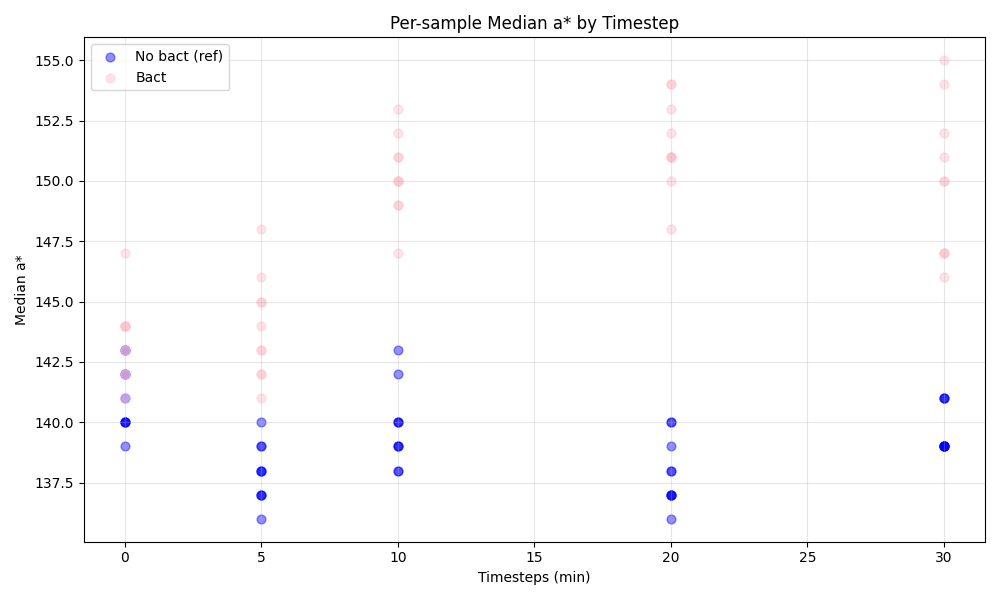
\includegraphics[width=0.48\textwidth]{results/statistical/control/control_no_norm.png}
\caption{Plot of the median $a^*$ for the FDBC control samples (without normalization).}
\label{fig:fdbc_no_norm}
\end{figure}

\begin{figure}[H]
\centering
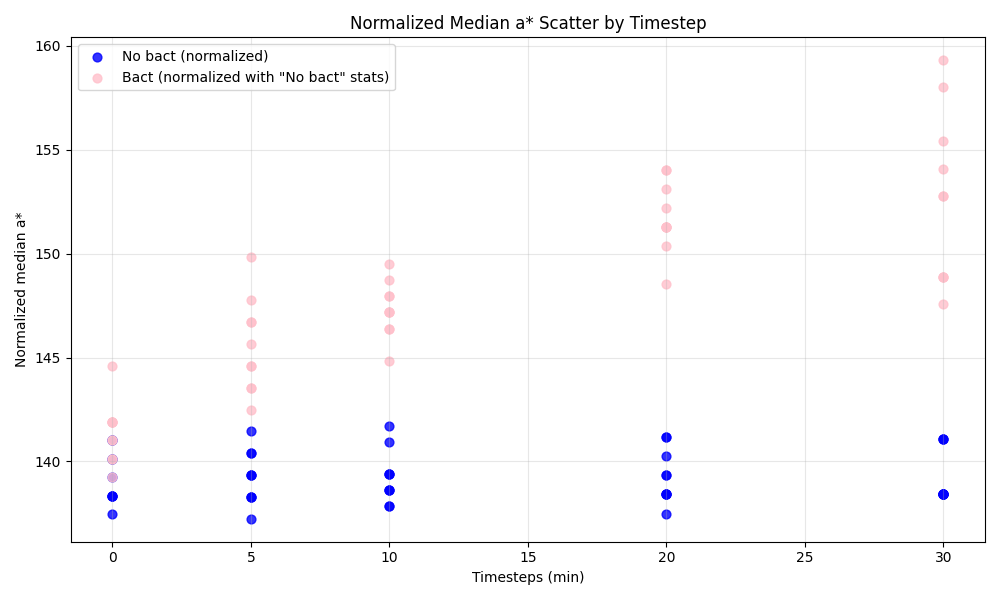
\includegraphics[width=0.48\textwidth]{results/statistical/control/control_norm.png}
\caption{Plot of the normalized median $a^*$ for the FDBC control samples.}
\label{fig:fdbc_norm}
\end{figure}

\subsubsection{Well-Plate Assays}
In the well-plate format, the normalized data proved robust enough to capture secondary colorimetric phenomena. We observed that prolonged exposure to light causes Resorufin to degrade, transitioning from pink to colorless in the growth control wells. This photobleaching effect is quantitatively tracked by our pipeline as a distinct drop in the normalized $a^*$ values after the 30th minute (see the orange dots in Fig. \ref{fig:wp_norm}).

At the 70-minute mark (see Fig. \ref{fig:wp_norm}), the pipeline successfully identifies bacterial growth, demonstrating significantly elevated $a^*$ values for the three lowest antibiotic concentrations, which aligns with the expected behavior of uninhibited strains.

Note that the plotted median $a^*$ values are obtained from averaging over the trials at each antibiotic concentration. Taking this average of 3 (each column) effectively suppresses localized anomalies (e.g., column 5 from the left, row 3, in Fig. \ref{fig:wp_sample}).

\begin{figure}[H]
\centering
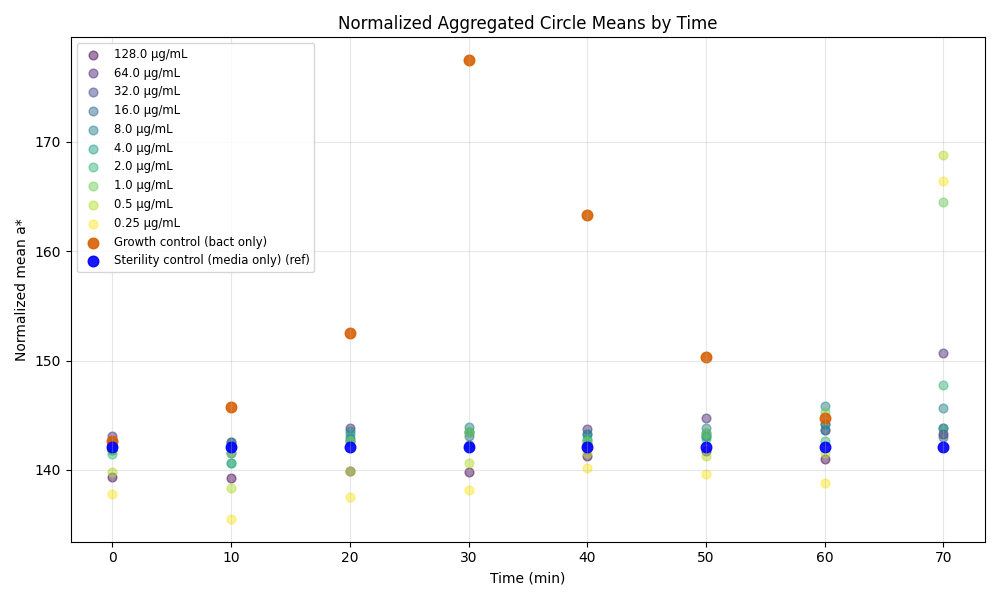
\includegraphics[width=0.48\textwidth]{results/statistical/well_plate/normalized_median_a_star_scatter_layout.png}
\caption{Plot of the normalized median $a^*$ (averaged over the trials at each antibiotic concentration) for the well-plate samples.}
\label{fig:wp_norm}
\end{figure}

\subsection{Statistical Significance}
The JSD tracking (Fig. \ref{fig:jsd}) confirms that the distribution shift becomes statistically significant as the experiment progresses. The JSD between the bacteria row and the control row increases over time, providing a clear window for automated decision-making.

\begin{figure}[H]
\centering
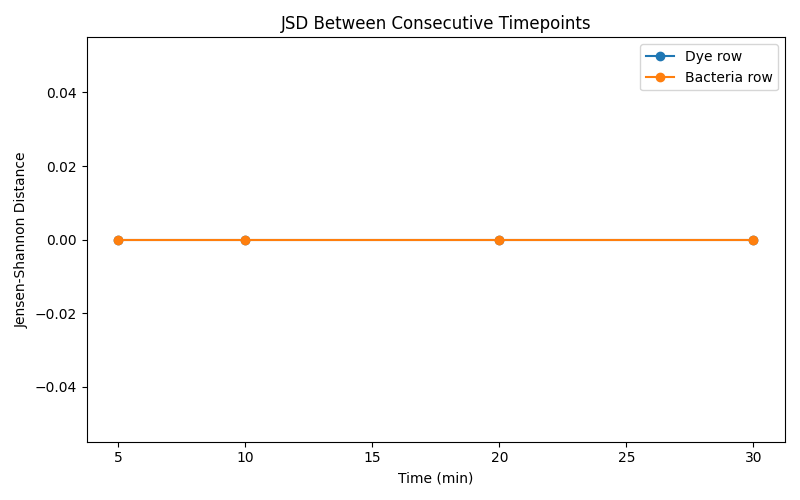
\includegraphics[width=0.48\textwidth]{results/statistical/jsd/jsd_over_time.png}
\caption{Jensen-Shannon Distance (JSD) tracking between consecutive timepoints for control and bacteria rows.}
\label{fig:jsd}
\end{figure}

\section{Inferences and Takeaways}
While the computer vision pipeline demonstrated technical success in segmentation and lighting normalization, the experimental transition to FDBC discs revealed significant physical and chemical challenges that hindered logical inferences.

\subsection{Substrate-Induced Inconsistency}
We observed that the FDBC discs did not yield consistent colorimetric patterns across repeated experiments. This inconsistency makes it difficult to establish a robust baseline for MIC determination on this specific substrate. 

\subsection{Percolation and Particle Size Dynamics}
A critical takeaway is the mismatch in physical distribution between the biological and chemical components:
\begin{itemize}
    \item \textbf{Surface Retention}: The bacteria, being larger biological entities, tend to remain trapped on the surface of the FDBC disc.
    \item \textbf{Downward Percolation}: The Resazurin dye and the antibiotic molecules are significantly smaller in particle size. Consequently, they percolate down into the porous structure of the cellulose substrate.
    \item \textbf{Reaction Hindrance}: This physical separation hinders the direct contact required for the redox reaction between the bacteria and the dye. It also creates non-uniform concentration dynamics for the antibiotic.
\end{itemize}

\subsection{Visual Quantification Artifacts}
The percolation effect leads to a non-uniform and patchy color distribution on the disc surface. This patchiness creates "perceived color" anomalies that mess up the median-based quantification of the CIELAB $a^*$ channel. Even with high-fidelity SAM masks, the statistical representation of a "patchy" disk is less reliable than a uniform liquid well, leading to noise that obscures the biological signal.

\section{Discussion}
The computer vision pipeline, utilizing SAM and CIELAB normalization, proved to be a powerful tool for standardizing AST analysis. It effectively removed environmental lighting noise and provided precise fluid isolation. However, the study highlights that the choice of substrate is as critical as the analytical method. 

The well-plate format provided clear, interpretable results and even allowed for the detection of secondary effects like photobleaching. In contrast, the FDBC format introduced physical variables---specifically percolation and surface-layer separation---that currently limit its diagnostic utility.

\section{Conclusion}
We have developed an AI-assisted colorimetric analysis pipeline for MIC determination that achieves reliable results in liquid-based well-plate assays. While the system effectively handles image acquisition and normalization challenges, its application to FDBC substrates is currently limited by non-uniform reaction dynamics and particle percolation. Future iterations must address these physical constraints, perhaps through substrate modification or different loading techniques, to fully realize the potential of point-of-care AST.

\section{Acknowledgments}
This work was completed as a final project for the course EE5360: Practical Challenges in Image Analysis at IIT Hyderabad.

\end{document}
